%%% Local Variables:
%%% mode: latex
%%% TeX-master: t
%%% End:
\documentclass{beamer}
\usepackage[utf8]{inputenc}
\usepackage[german]{babel}
\usepackage{graphics}
\usepackage{listings}
\usepackage{caption}

\captionsetup{font=scriptsize,labelfont=scriptsize}

\usetheme{default}
\usecolortheme{rose}

\DeclareGraphicsRule{.pdftex}{pdf}{.pdftex}{}

% \lstdefinelanguage{cfengine}
%   {morekeywords={import,classes,control,admit,copy,editfiles,processes,shellcommands},
%    sensitive=false,
%    morecommment[l]{//},
%   }

\newcommand\Fontvi{\fontsize{6}{7.2}\selectfont}

\lstset{
basicstyle=\tiny,
stringstyle=\tiny,
numbers=left,
numberstyle=\tiny,
stepnumber=2,
frame=single,
%language=cfengine,
captionpos=b
}

\title{System Automation mit Puppet und Foreman\\}
\author{Toni Schmidbauer}

\begin{document}

\begin{frame}
\center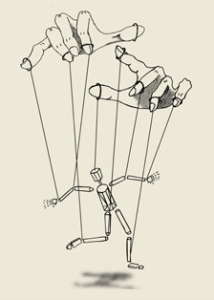
\includegraphics[height=2.5cm,width=2cm]{../pics/puppet.png}
\titlepage

\end{frame}

\begin{frame}
  \frametitle{whoami}
  \begin{itemize}
  \item SysAdmin@s-itsolutions
  \item toni@stderr.at
  \item \url{http://stderr.at}
  \item \url{http://github.com/tosmi}
  \item stderr@jabber.org
  \end{itemize}
\end{frame}
\begin{frame}

  \frametitle{Agenda}

  \begin{itemize}
  \item Kurze Umfrage
  \item Was ist Puppet?
  \item Was ist Foreman?
  \item Puppet@s-iTSolutions
  \item Was haben wir geplant?
  \end{itemize}

\end{frame}

\begin{frame}
\center{\huge{Umfrage}}
\end{frame}

\begin{frame}[fragile]
  \frametitle{Was ist Puppet?}

  \begin{itemize}
  \item Declarative programming: telling the machine what you would
    like to happen, and let the computer figure out how to do it.
  \item \tiny{Imperative programming: telling the machine how to do
    something}
  \end{itemize}

  \begin{lstlisting}
    class linuxwochen2014 (
      $ensure = present
    ) {
      user { 'toni':
        ensure => $ensure,
        uid    => 4711,
        gid    => 100,
      }

      package { 'emacs-nox':
        ensure => installed
      } ->
      package { 'vim-enhanced':
        ensure => absent,
      }
    }
  \end{lstlisting}
\end{frame}


\begin{frame}[fragile]
  \frametitle{Zuordnung von Klassen}

  \begin{itemize}
    \item über manifests/site.pp
      \begin{lstlisting}
        node /^(foo|bar)\.linuxwochen\.at$/ {
          class { 'linuxwochen2014':
            ensure => absent
          }
        }
      \end{lstlisting}
  \item über Hiera (hiera\_include('classes',[````]))
  \item über einen External Node Classifier (Foreman)
  \end{itemize}
\end{frame}


\begin{frame}[fragile]
  \frametitle{Node classification}
\begin{lstlisting}
---
classes:
  black:
  puppetmgmt:
    manage_config: true
    puppetmaster: puppetd
    puppet_version: 3.2.4
  sudo:
    config_dir: /etc/sudoers.d/
    config_file: /etc/sudoers
    config_file_replace: false
    package: sudo
    package_source: ''
    purge: false
\end{lstlisting}
\end{frame}

\begin{frame}[fragile]
  \frametitle{Puppet Environments}
  \begin{itemize}
  \item Environments sind unabhängige Puppet Umgebungen
  \item Ein Master kann mehrere Environments zur Verfügung stellen
  \end{itemize}

\begin{lstlisting}
/etc/puppet/modules/...
/etc/puppet/manifests/site.pp

/etc/puppet/environments/linuxwochen/modules
/etc/puppet/environments/linuxwochen/manifests/site.pp
\end{lstlisting}
\end{frame}

\begin{frame}
  \frametitle{Was ist Foreman?}
  \begin{figure}[ht]
    \centering
    \framebox{
      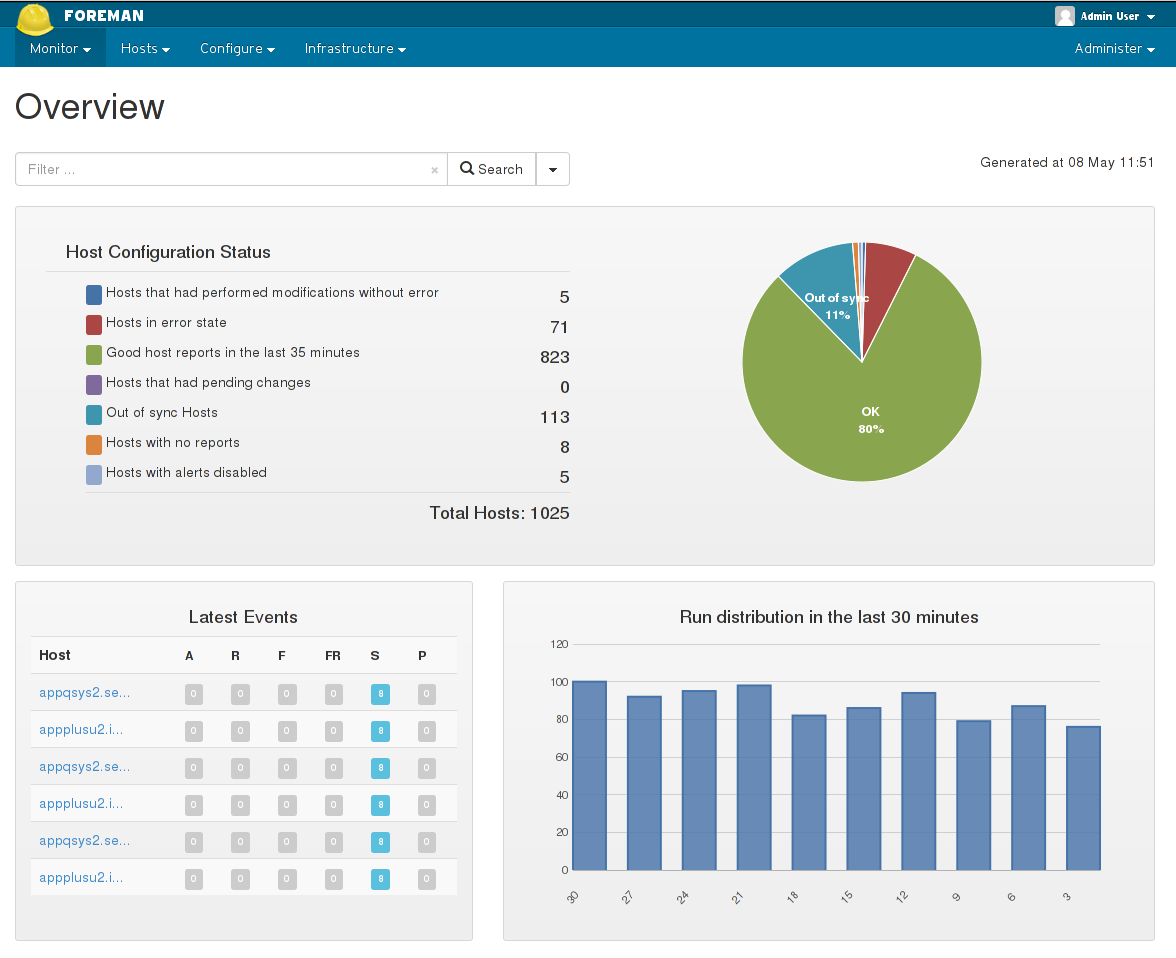
\includegraphics[height=7.5cm,width=10.3cm]{../pics/foreman_dashboard.png}
    }
    \label{fig:stack}
  \end{figure}
\end{frame}

\begin{frame}
  \frametitle{Puppet run}
  \begin{figure}[ht]
    \centering
      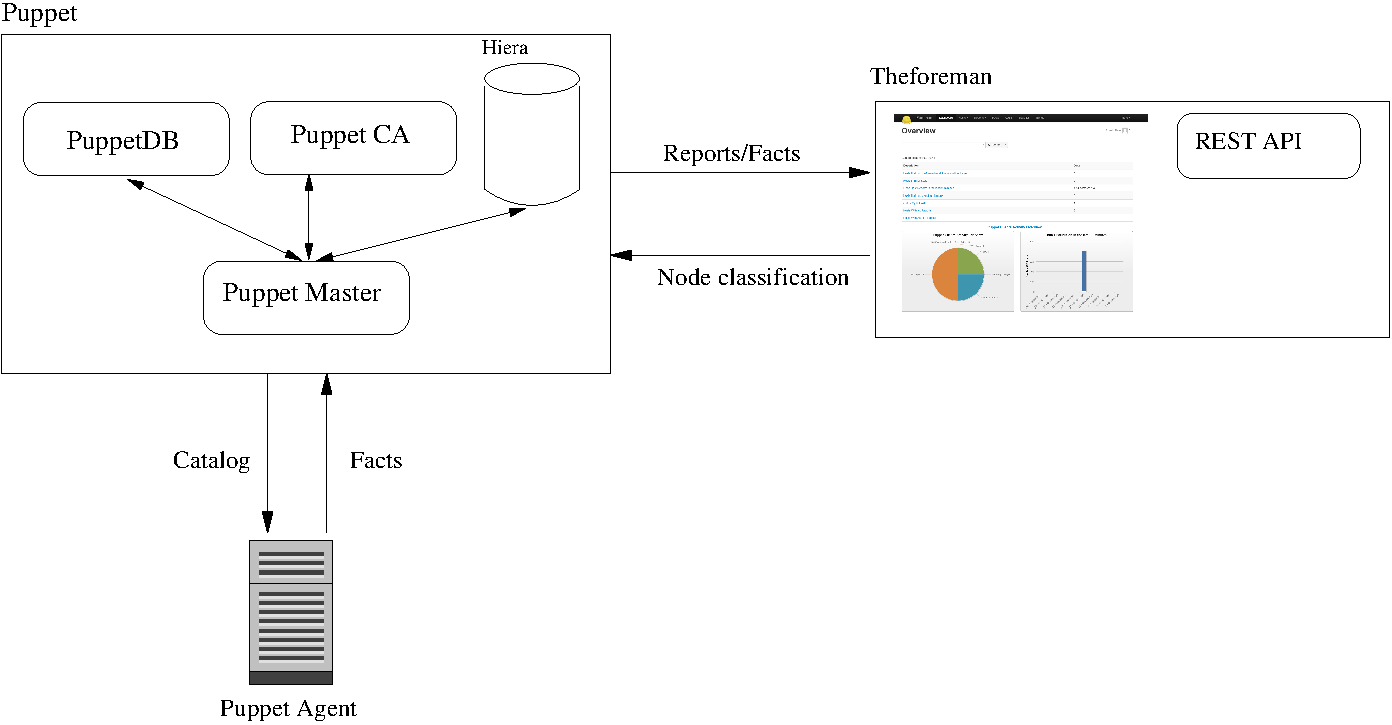
\includegraphics[height=6cm,width=11cm]{../pics/puppet_overview}
    \label{fig:stack}
  \end{figure}
\end{frame}

\begin{frame}
  \center{\huge{Und jetzt?}}
\end{frame}

\begin{frame}
  \begin{figure}[ht]
    \centering
      
\includegraphics[height=7.5cm,width=10cm]{../pics/chucky.png}
    \label{fig:stack}
  \end{figure}
\end{frame}

\begin{frame}
  \begin{itemize}
  \item Wie soll eine Entwicklungsumgebung aussehen?
  \item Wie testen wir den Puppet Code?
  \item Wie verwalten wir unseren Puppet Code?
  \item Wie soll unsere Puppet Umgebung aussehen?
  \item Wie erfolgt das Deployment des Codes?
  \item Wie verwalten wir Module von PuppetForge?
  \end{itemize}
\end{frame}

\begin{frame}
  \center{\huge{Wie soll eine Entwicklungsumgebung aussehen?}}
\end{frame}

\begin{frame}
  \frametitle{Vagrant}

  \begin{itemize}
  \item \url{http://vagrantup.com}
  \item Ermöglicht virtuelle Entwicklungsumgebungen
  \item Vagrant Box ist ein vorkonfiguriertes Image
  \item Default VirtualBox andere Provider via Plugins (VMWare, KVM)
  \end{itemize}
\end{frame}

\begin{frame}
  \center{\huge{Demo}}
\end{frame}

\begin{frame}
  \center{\huge{Wie testen wir den Puppet Code?}}
\end{frame}

\begin{frame}[fragile]
  \frametitle{rspec-puppet}

  \begin{itemize}
  \item Ruby RSpec Tests für Puppet
  \item Jedes Module muss RSpec Tests mitbringen
  \end{itemize}

  \begin{lstlisting}
require 'spec_helper'
describe 'linuxwochen2014' do
  let :facts { { :osfamily => 'RedHat' } }

  context 'ensure is set to absent' do
    let :params { { :ensure => 'absent'} }

    it do
      should contain_user('toni').with({
                                         'ensure' => 'absent',
                                         'uid'    => '4711',
                                         'gid'    => '100',
                                      })
    end

    it { should contain_package('emacs-nox').with_ensure('installed') }
    it { should contain_package('vim-enhanced').with_ensure('absent') }
    it { should contain_package('emacs-nox).that_comes_before('Package[vim-enhanced]') }
  end
end
  \end{lstlisting}

\end{frame}

\begin{frame}
  \center{\huge{Demo}}
\end{frame}

\begin{frame}
  \center{\huge{Wie verwalten wir unseren Puppet Code?}}
\end{frame}

\begin{frame}
  \frametitle{GIT}

  \begin{itemize}
  \item Ein zentrales GIT Repository
  \item 3 Hauptbranches
    \begin{itemize}
    \item Master
    \item Testing
    \item Production
    \end{itemize}
  \item Feature Branches für neue Module
  \item Berechtigungssystem mit Gitolite
  \end{itemize}
\end{frame}

% \begin{frame}
%   \center{\huge{Demo}}
% \end{frame}

\begin{frame}
  \center{\huge{Wie soll unsere Puppet Umgebung aussehen?}}
  \center{\huge{Wie erfolgt das Deployment des Codes?}}
\end{frame}

\begin{frame}
  \frametitle{Umgebungen}

    \begin{itemize}
    \item Development (Master)
      \begin{itemize}
      \item Test auf 7 Entwicklungsserver
      \item Push auf Remote Master Branch löst Deployment aus
      \item RedHat 5,6 / Solaris {sparc,i386} {10,11} / AIX
      \end{itemize}
    \item Testing
      \begin{itemize}
      \item ca. 30 ``Produktions'' Server
      \item Annotated Tags werden automatisch deployed (test\_*)
      \end{itemize}
    \item Production
      \begin{itemize}
      \item ca 1000 Hosts
      \item Annotated Tags werden automatisch deployed (prod\_*)
      \end{itemize}
    \end{itemize}
\end{frame}

\begin{frame}
  \frametitle{Jenkins CI}

  \begin{itemize}
  \item Continuous Integration Server
  \item Führt Jobs aus (z.b. Shell Scripts)
  \item Monitored und liefert Status Jobs
  \item Es können Abhängigkeiten zwischen Jobs definiert werden
  \end{itemize}
\end{frame}

\begin{frame}
  \frametitle{Puppet Umgebung und Deployment}
  \begin{figure}[ht]
    \centering
      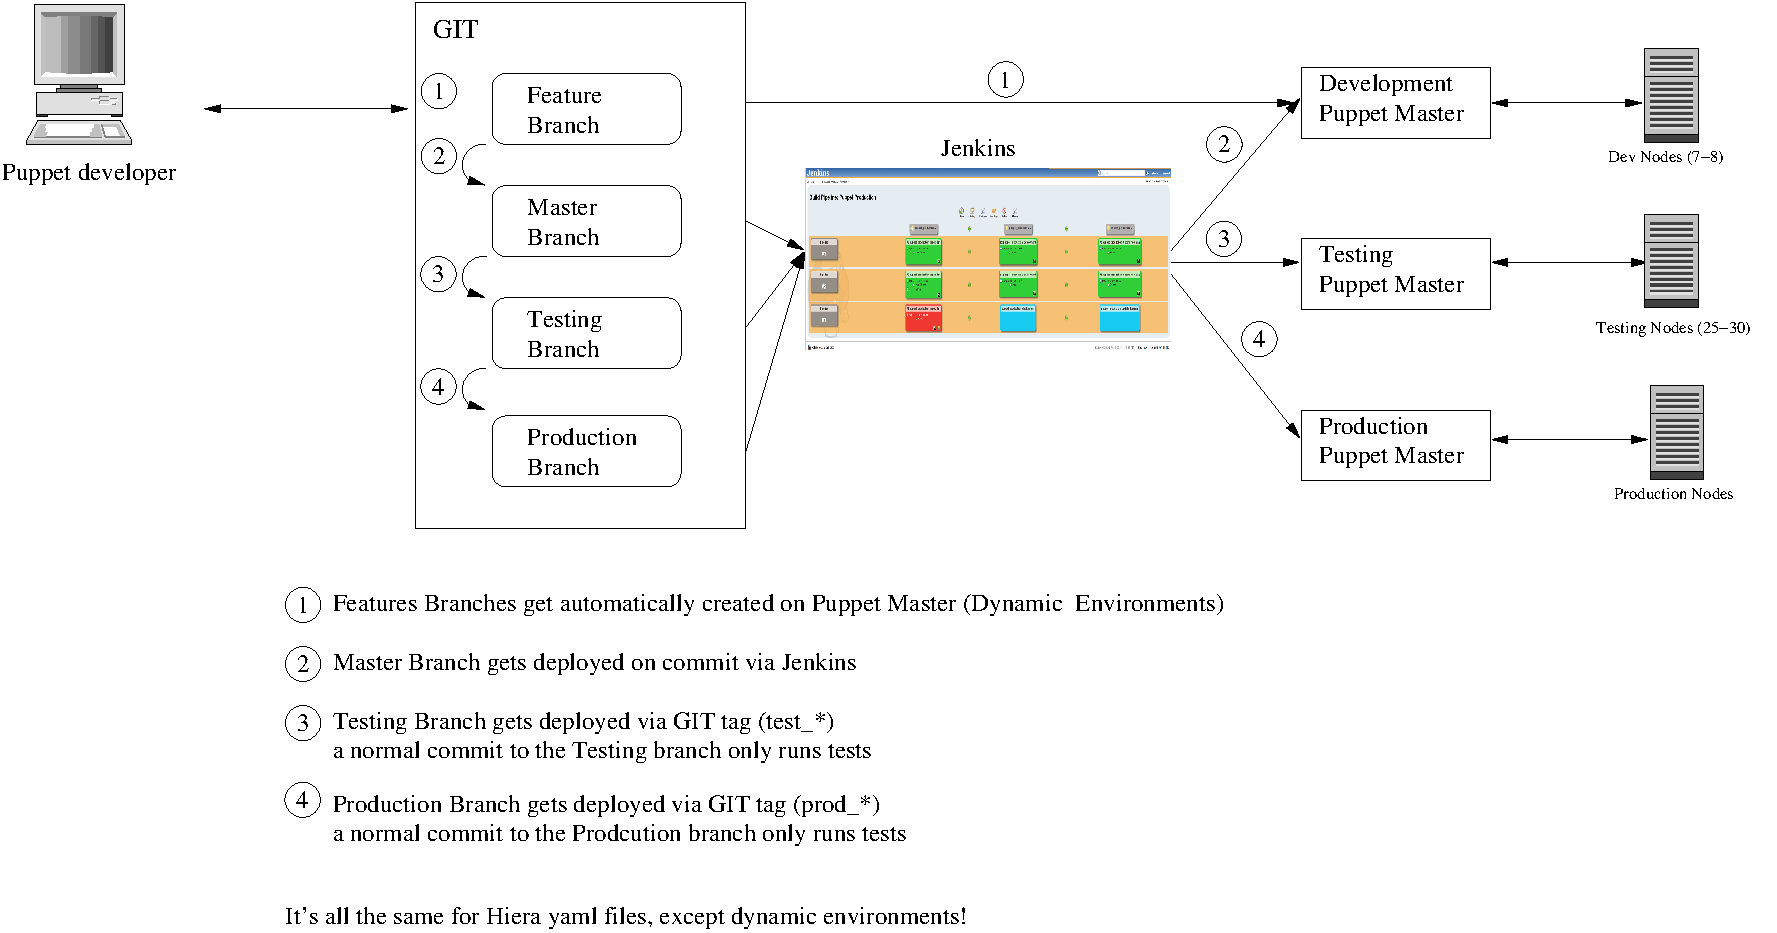
\includegraphics[height=5.5cm,width=11cm]{../pics/puppet_deployment2}
  \end{figure}
\end{frame}

\begin{frame}
  \frametitle{Deployment}
  \begin{figure}[ht]
    \centering
      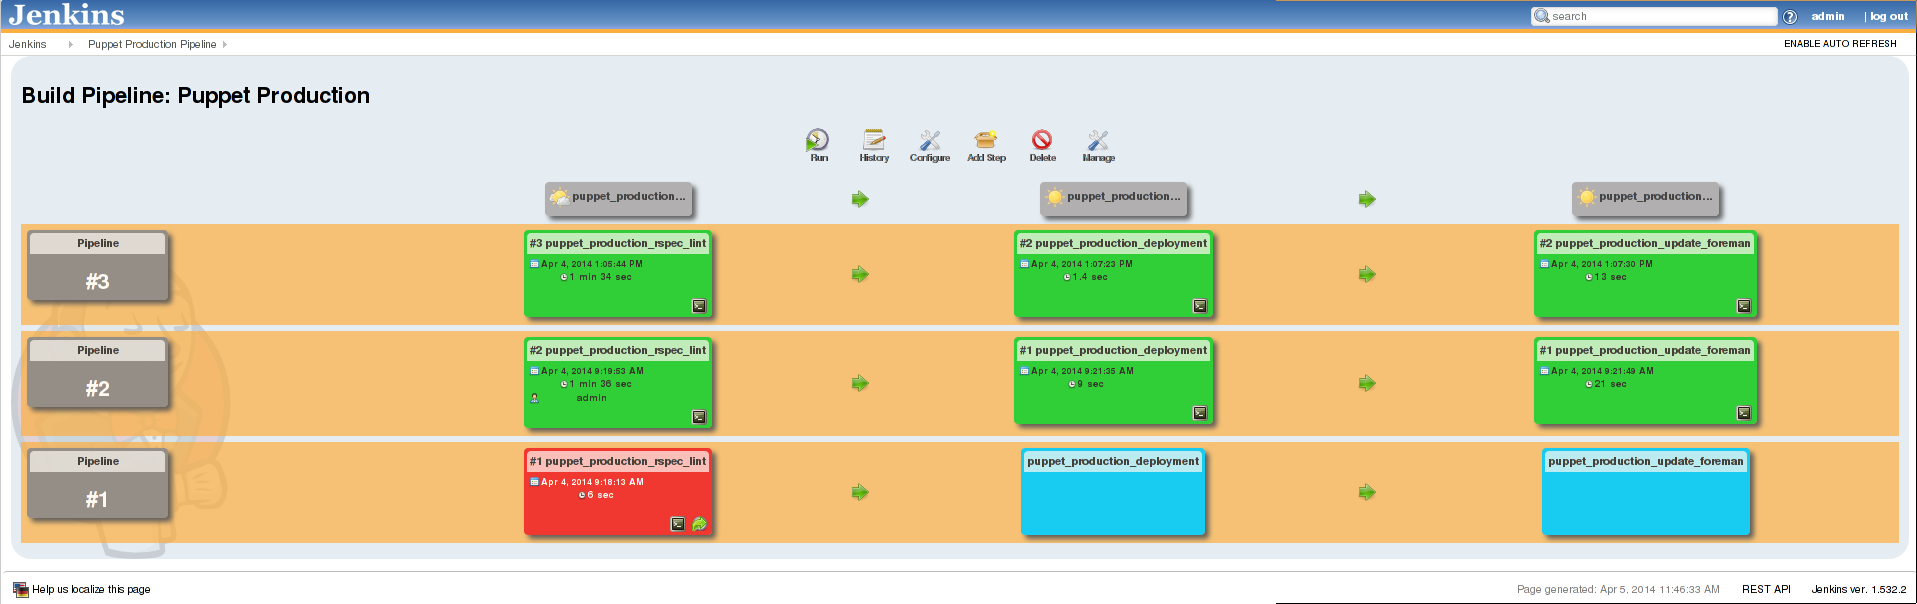
\includegraphics[height=5cm,width=11cm]{../pics/jenkins_pipeline}
    \label{fig:stack}
  \end{figure}
\end{frame}

\begin{frame}
  \frametitle{Monitoring}
  \begin{figure}[ht]
    \centering
      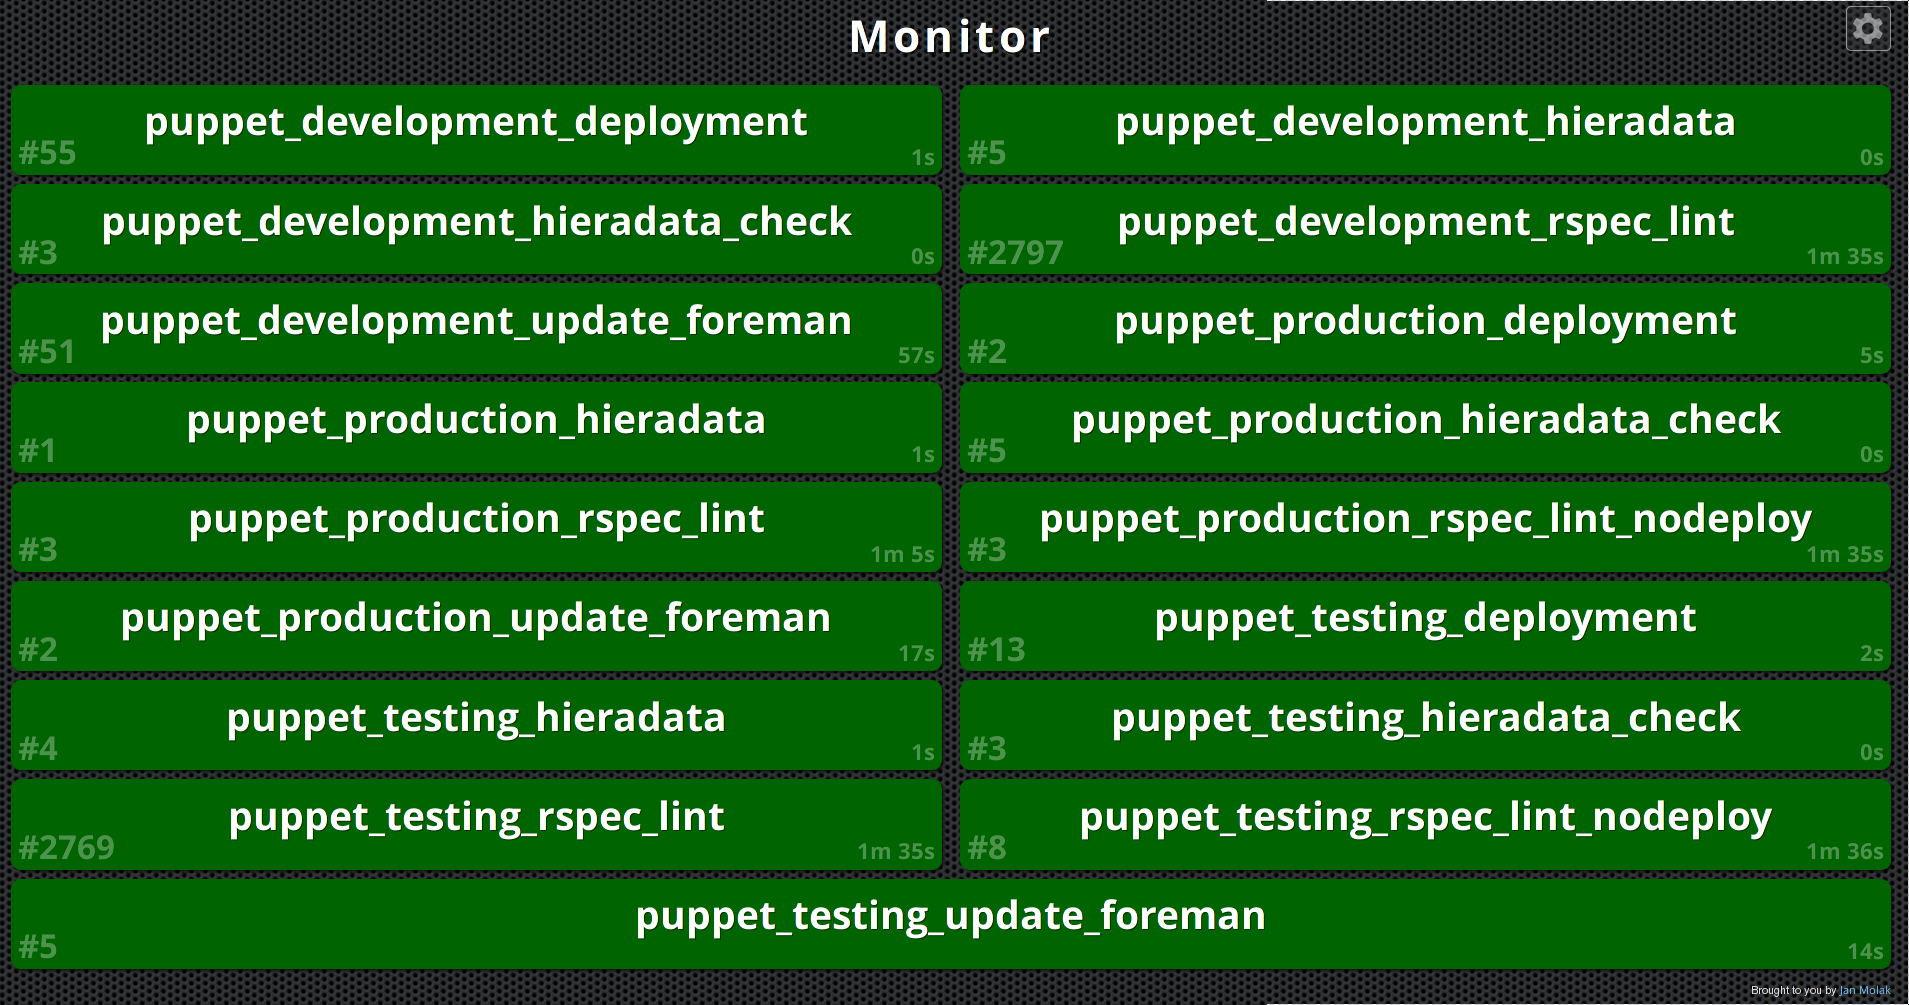
\includegraphics[height=6cm,width=11cm]{../pics/jenkins_monitor.png}
    \label{fig:stack}
  \end{figure}
\end{frame}


\begin{frame}
  \center{\huge{Wie verwalten wir Module von PuppetForge?}}
\end{frame}

\begin{frame}
  \frametitle{Puppetforge Module}

  \begin{itemize}
  \item Eigenes GIT Repository (puppetforge.git)
  \item Download der Module in der Enwicklungsumgebung via \\ \texttt{puppet module install ...}
  \item Staging GIT pull (bäh!)
  \item Dies ändert sich allerdings (dazu später)
  \end{itemize}
\end{frame}

\begin{frame}
  \begin{itemize}
  \item Wie soll eine Entwicklungsumgebung aussehen? \emph{\color{green}DONE}
  \item Wie testen wir den Puppet Code? \emph{\color{green}DONE}
  \item Wie verwalten wir unseren Puppet Code? \emph{\color{green}DONE}
  \item Wie soll unsere Puppet Umgebung aussehen?  \emph{\color{green}DONE}
  \item Wie erfolgt das Deployment des Codes? \emph{\color{green}DONE}
  \item Wie verwalten wir Module von PuppetForge? \emph{\color{green}DONE}
  \end{itemize}
\end{frame}

\begin{frame}
  \begin{figure}[ht]
    \centering
      
\includegraphics[height=6cm,width=10cm]{../pics/puppy.png}
    \label{fig:stack}
  \end{figure}
\end{frame}

\begin{frame}
  \frametitle{Probleme, Probleme, Probleme...}

  \begin{itemize}
  \item Ein GIT Repo funktioniert nicht bei Änderungen von Upstream Modulen
  \item Andere Abteilungen sollen ihre Module unabhänging testen
  \item Unittests sagen noch nichts aus wie sich der Code am Live-System verhält
  \item Wir sollten eigentlich das Zusammenspiel aller Module testen (Forge und eigene)
  \end{itemize}
\end{frame}

\begin{frame}
  \frametitle{Was haben wir geplant?}

  \begin{itemize}
  \item r10k für Deployment (\url{https://github.com/adrienthebo/r10k})
  \item Ein Repository pro Module
  \item Nur interne Module bleiben im Hauptrepo
  \item Acceptance Tests mit Beaker
  \end{itemize}
\end{frame}

\begin{frame}
  \frametitle{Links und Bücher}
\tiny
  \begin{itemize}
  \item \url{http://github.com/tosmi/linuxwochen2014}
  \item \url{http://github.com/tosmi/puppet-devel}
  \item Puppet Learning VM: \url{http://puppetlabs.com/download-learning-vm}
  \item Foreman: \url{http://theforeman.org}
  \item Vagrant: \url{http://vagrantup.com}
  \item rspec-puppet: \url{http://rspec-puppet.com/}
  \item puppet-lint: \url{http://puppet-lint.com/}
  \item Gitolite: \url {http://gitolite.com/}
  \item r10k: \url{https://github.com/adrienthebo/r10k}
  \item Roles and Profiles: \url{http://www.craigdunn.org/2012/05/239/}
  \item Dynamische Puppet Umgebungen: \url{http://puppetlabs.com/blog/git-workflow-and-puppet-environments}
  \item puppet-sync: \url{https://github.com/pdxcat/puppet-sync}
  \item \texttt{Instant Puppet 3 Starter}
  \item \texttt{Pro Puppet 2nd}
  \item \texttt{The RSpec Book}
  \item \texttt{Pulling Strings with Puppet}
  \item \texttt{Continuous Delivery}
  \end{itemize}
\end{frame}

\begin{frame}
  \huge{Danke für die Aufmerksamkeit}
\end{frame}
\end{document}


todo

kann puppet ueber proxy kommunizieren? ja
exported resources...
vagrant beispiel
